% linear_workflow.tex - 线性科研技术路线图模板 (Linear Workflow Schematic)
% 编译方式: pdflatex linear_workflow.tex 或 xelatex linear_workflow.tex
\documentclass[tikz,border=10pt]{standalone}
\usepackage{xcolor}
\usepackage{tikz}
\usetikzlibrary{arrows.meta, positioning, calc, shapes.geometric, backgrounds, fit}

% 顶刊标准色定义 (与 assets/palettes.json 严格对应)
\definecolor{natureblue}{HTML}{4E79A7}
\definecolor{natureorange}{HTML}{F28E2B}
\definecolor{naturered}{HTML}{E15759}
\definecolor{naturecyan}{HTML}{76B7B2}
\definecolor{naturegreen}{HTML}{59A14F}
\definecolor{darktext}{HTML}{262626}
\definecolor{subtext}{HTML}{6C757D}
\definecolor{lightbg}{HTML}{F8F9FA}
\definecolor{boxborder}{HTML}{CBD5E1}

\begin{document}
\sffamily
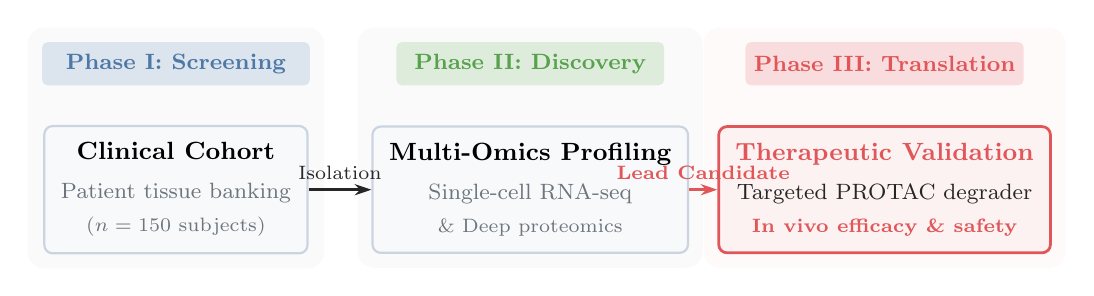
\begin{tikzpicture}[
    node distance=1.2cm and 1.8cm,
    % 基础流程节点样式
    stagebox/.style={
        rectangle,
        rounded corners=3pt,
        draw=boxborder,
        fill=lightbg,
        line width=0.8pt,
        minimum width=3.2cm,
        minimum height=1.6cm,
        inner sep=6pt,
        align=center
    },
    % 终点高亮节点
    highlightbox/.style={
        stagebox,
        draw=naturered,
        fill=naturered!8,
        line width=1.0pt
    },
    % 阶段分类横幅
    phasebanner/.style={
        rectangle,
        rounded corners=2pt,
        inner sep=3pt,
        font=\bfseries\footnotesize,
        align=center,
        minimum height=0.55cm
    },
    % 激活连线箭头
    steparrow/.style={
        -{Stealth[length=6pt,width=4pt]},
        line width=1.0pt,
        color=darktext
    },
    % 强调连线
    accentarrow/.style={
        steparrow,
        color=naturered
    }
]

    % --- 阶段横幅 (顶部) ---
    \node[phasebanner, fill=natureblue!20, text=natureblue, minimum width=3.4cm] (p1) at (0, 1.6) {Phase I: Screening};
    \node[phasebanner, fill=naturegreen!20, text=naturegreen, minimum width=3.4cm] (p2) at (4.5, 1.6) {Phase II: Discovery};
    \node[phasebanner, fill=naturered!20, text=naturered, minimum width=3.4cm] (p3) at (9.0, 1.6) {Phase III: Translation};

    % --- 核心流程节点 ---
    % Step 1
    \node[stagebox] (s1) at (0, 0) {
        {\bfseries\small Clinical Cohort}\\[2pt]
        {\footnotesize\color{subtext} Patient tissue banking}\\
        {\scriptsize\color{subtext} ($n = 150$ subjects)}
    };

    % Step 2
    \node[stagebox] (s2) at (4.5, 0) {
        {\bfseries\small Multi-Omics Profiling}\\[2pt]
        {\footnotesize\color{subtext} Single-cell RNA-seq}\\
        {\scriptsize\color{subtext} \& Deep proteomics}
    };

    % Step 3
    \node[highlightbox] (s3) at (9.0, 0) {
        {\bfseries\small\color{naturered} Therapeutic Validation}\\[2pt]
        {\footnotesize\color{darktext} Targeted PROTAC degrader}\\
        {\scriptsize\color{naturered}\bfseries In vivo efficacy \& safety}
    };

    % --- 连接箭头与标注 ---
    \draw[steparrow] (s1) -- node[above, font=\scriptsize\color{subtext}] {Isolation} (s2);
    \draw[accentarrow] (s2) -- node[above, font=\scriptsize\color{naturered}\bfseries] {Lead Candidate} (s3);

    % --- 阶段边界框 (可选背景) ---
    \begin{scope}[on background layer]
        \node[draw=none, fill=gray!4, rounded corners=6pt, fit=(p1)(s1), inner sep=5pt] {};
        \node[draw=none, fill=gray!4, rounded corners=6pt, fit=(p2)(s2), inner sep=5pt] {};
        \node[draw=none, fill=naturered!3, rounded corners=6pt, fit=(p3)(s3), inner sep=5pt] {};
    \end{scope}

\end{tikzpicture}
\end{document}
